\chapter{Conclusão}\label{cap:conclusao}

A tarefa de se encontrar vagas em estacionamentos tem se tornado cada vez mais difícil com o aumento da frota de veículos das grandes cidades. Essa busca por um espaço livre para estacionar o carro pode durar muito tempo, criando gastos que se acumulam até valores altíssimos.

Buscando minimizar estes problemas, diversos sistemas de mapeamento de estacionamento e detecção de vagas livres foram desenvolvidos. Algumas soluções são implementadas nos próprios veículos \cite{schmid2011parking}, mas as mais interessantes para uma solução geral do problema são aquelas que detectam a quantidade de vagas livres em uma região do estacionamento e disponibilizam essa informação para todos os seus usuários. Em garagens, sensores de vários tipos podem ser utilizados \cite{kianpisheh2012smart,lee2008intelligent,wolff2006parking}, mas estas soluções não são muito adequadas para aplicação em estacionamentos descobertos. 

Para estes casos, uma solução que se mostrou adequada e de fácil implementação foi o uso de câmeras de vídeo e algoritmos de processamento de imagens e visão computacional. Este trabalho apresentou um algoritmo para ser utilizado em um sistema como estes, chamado de \textit{Detector de vagas em estacionamentos abertos}, abreviado como \textit{DVE}. O algoritmo recebe as imagens de câmera de vídeo coloridas montadas em postes de luz e usa uma rede neural artificial combinada com uma técnica de rastreamento dos veículos através do fluxo óptico para mapear e determinar a ocupação das vagas que aparecem na imagem.

O \textit{DVE} é especialmente adequado para estacionamentos descobertos com postes de luz em intervalos de distância regular e com poucas ou nenhuma obstrução visual. Quando testado em vídeos que simulavam a captura de uma câmera instalada em um destes postes, o programa apresentou resultados bastante semelhantes a resultados determinados por um observador humano. O \textit{DVE} apresentou dificuldade em classificar corretamente regiões ocupadas por carros com coloração semelhante a do asfalto quando iluminados de certa maneira. Além disso apresentou a possibilidade de detecção errônea de vagas, o que fazia que fossem acusadas uma ocupação maior do que a real nos vídeos.

Apesar de alguns erros, o \textit{DVE} é resistente a pequenos erros de classificação da rede neural na maioria dos casos e até aos movimentos do equipamento de captura, já que na maioria das vezes continuou detectando o número correto de vagas ocupadas na imagem apesar destes empecilhos.

Por fim, o programa se mostrou promissor e capaz de ajudar de forma simples usuários de estacionamento a encontrarem vagas com mais facilidade. Ainda é necessário, porém, fazer um refinamento do sistema de mapeamento do \textit{DVE}, de forma que seja possível criar um mapa mais preciso do estacionamento monitorado e disponibilizar mais informações aos usuários, como o tempo médio de espera ou a posição exata das vagas livres. Um outro possível trabalho futuro é uma adaptação do \textit{DVE} que o torne capaz de funcionar com imagens de câmeras em ângulos oblíquos ao estacionamento, permitindo uma instalação ainda mais fácil e em estacionamentos de tipos mais variados. Já foram feitos experimentos neste sentido usando seções quadradas menores ao invés das seções verticais utilizadas atualmente e a mesma rede neural com resultados premilinares promissores, como exemplificado na Figura \ref{fig:preliminares}.

\begin{figure}%
\centering
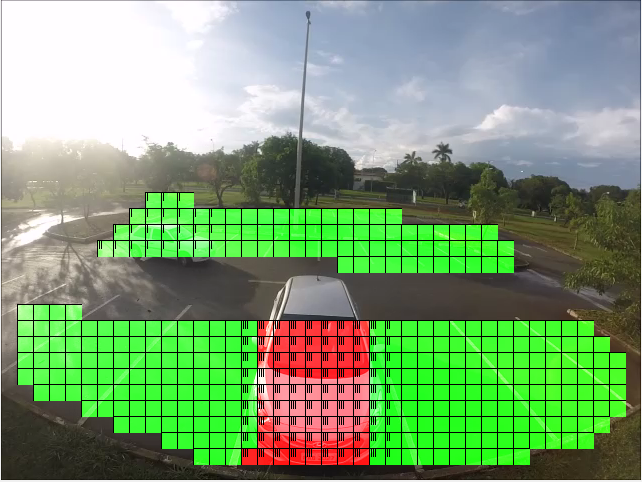
\includegraphics[width=8cm]{preliminar}%
\caption{Resultados preliminares de um possível trabalho futuro.}%
\label{fig:preliminares}%
\centering
\end{figure}









